% Book 4, Year 2, chapter 24 -- Predicate logic and formal proofs.
% Provenance (never printed): sources/book4/BRIEFS.md, chapter 24.
\chapter{Predicate Logic and Formal Proofs}\label{ch:b2:predicate-logic}

The town library has rules: a person with a book out is a member, a book is out to one person at most, every member
has a friend. Each one speaks of \emph{all} the people and \emph{some} book, which propositional formulas
cannot say. Written in a language with \omterm{def:b2:predicate-logic:formula}{quantifiers}, the rules can be checked against the town's tables by a program:

\omcode{code/bachelor-2/24-predicate-logic/listings/evaluate.py}{5}{27}{Five rules about the library as formulas, each
evaluated on the town's tables, with the first counterexamples found}\label{lst:b2:predicate-logic:evaluate}

\omoutput{code/bachelor-2/24-predicate-logic/outputs/evaluate.txt}{Three rules hold; two fail. Four books are recorded as
out to two people at once, and 41 members have no friend in the friendships table.}\label{out:b2:predicate-logic:evaluate}

A check on the data says what holds \emph{today}. Some rules hold for a better reason: they follow from others, in
every possible town. If whoever has a book out is a member, and every member may borrow, then whoever has a book out
may borrow, whatever the tables contain. This chapter defines the language of such rules, what it means for a formula
to be true in a \omterm{def:b2:predicate-logic:structure}{structure}, and proofs: trees of small steps, each checked mechanically, with a theorem that a proved
formula is true wherever its hypotheses are. It ends with two algorithmic tools of logic, unification and resolution,
and a linear-time algorithm for 2-SAT.

\begin{recall}
The Year 1 volume: propositional formulas as trees, valuations, a \omterm{def:b2:predicate-logic:consequence}{model} of a formula, satisfiability, logical
consequence and equivalence; literals, clauses and CNF; the satisfiability problem and $k$-SAT; strongly connected
components of a directed graph, and Kosaraju's algorithm, which finds them with two depth-first searches in linear time;
structural induction. From mathematics: sets, relations, functions, tuples.
\end{recall}

\section{Syntax: terms, formulas, variables}\label{sec:b2:predicate-logic:syntax}

\begin{definition}[First-order signature, term, atomic formula]\label{def:b2:predicate-logic:term}
A \emph{first-order signature}\index{first-order signature} is a set of \emph{function symbols} and a set of
\emph{predicate symbols}, each with an \emph{arity}, its number of arguments; a function symbol of arity $0$ is a
\emph{constant}. Given an infinite set of \emph{variables}, the \emph{terms}\index{term (logic)} are built by: a variable
is a term; if $f$ has arity $n$ and $t_1, \dots, t_n$ are terms, $f(t_1, \dots, t_n)$ is a term. An \emph{atomic
formula}\index{atomic formula} is $P(t_1, \dots, t_n)$ for a predicate symbol $P$ of arity $n$, an equality $t_1 = t_2$,
or $\bot$ (false).
\end{definition}

The library's signature has the constants \code{p5}, \code{b3}, \dots, the predicates $\mathit{Person}$,
$\mathit{Member}$ and $\mathit{Book}$ of arity 1, and $\mathit{Out}$, $\mathit{Borrowed}$ and $\mathit{Friend}$ of arity
2. Arithmetic has the constant $0$, the successor $s$ of arity 1 and $+$ of arity 2, so $s(0) + x$ is a term. A term
names an object; an \omterm{def:b2:predicate-logic:term}{atomic formula} says something about objects, and is true or false.

\begin{definition}[First-order formula, quantifier]\label{def:b2:predicate-logic:formula}
The \emph{first-order formulas}\index{first-order formula} are built by: an \omterm{def:b2:predicate-logic:term}{atomic formula} is a formula; if $A$ and $B$
are formulas and $x$ is a variable, $\neg A$, $A \wedge B$, $A \vee B$, $A \to B$, $\forall x\, A$ and $\exists x\, A$
are formulas. The symbols $\forall$ (\emph{for all}) and $\exists$ (\emph{there exists}) are the
\emph{quantifiers}\index{quantifier}. \emph{Predicate logic}\index{predicate logic} is the study of these formulas.
\end{definition}

As in the Year 1 volume, a formula is a tree, and brackets are only a way to write it on a line. The conventions
are: $\neg$ binds tightest, then $\wedge$, $\vee$ and $\to$, which groups to the right; a \omterm{def:b2:predicate-logic:formula}{quantifier} reaches as far
right as possible, so $\forall x\, P(x) \to Q(x)$ is $\forall x\, (P(x) \to Q(x))$. The listings write \code{~},
\code{&}, \code{|}, \code{->}, \code{forall x.} and \code{exists x.}, and the library \code{formulas.py} reads and prints
that text; its parser treats the names $u$ to $z$, possibly followed by digits, as variables, and other lower-case names
as constants.

\begin{definition}[Free variable, bound variable, scope]\label{def:b2:predicate-logic:free}
In $\forall x\, A$ and $\exists x\, A$, the formula $A$ is the \emph{scope}\index{scope (quantifier)} of the \omterm{def:b2:predicate-logic:formula}{quantifier}.
An occurrence of $x$ is \emph{bound}\index{bound variable} if it lies in the scope of a \omterm{def:b2:predicate-logic:formula}{quantifier} on $x$, and then it
is bound by the nearest such \omterm{def:b2:predicate-logic:formula}{quantifier} above it in the tree; otherwise it is \emph{free}\index{free variable}. The
free variables of a formula are those with a free occurrence; a formula without any is a
\emph{sentence}\index{sentence (logic)}.
\end{definition}

The \omterm{def:b2:predicate-logic:free}{free variables} are computed by structural induction, one line per case:

\omcode{code/bachelor-2/24-predicate-logic/listings/formulas.py}{66}{80}{The \omterm{def:b2:predicate-logic:free}{free variables} of a term or a formula; a
\omterm{def:b2:predicate-logic:formula}{quantifier} removes its own variable}\label{lst:b2:predicate-logic:free}

A formula's truth depends on its \omterm{def:b2:predicate-logic:free}{free variables}, as $x < 3$ depends on $x$; a \omterm{def:b2:predicate-logic:free}{sentence} is simply true or false in a
given world. In $\forall x\, (R(x, y) \to \exists x\, P(x))$, the first $x$ is \omterm{def:b2:predicate-logic:free}{bound} by $\forall x$, the second by
$\exists x$, and $y$ is \omterm{def:b2:predicate-logic:free}{free}:

\begin{omfigure}
\begin{forest}
for tree={font=\small, l sep=8pt, s sep=14pt}
[$\forall x$, name=fa
  [$\to$
    [$R$ [$x$, name=x1] [$y$, name=y1, draw, circle, inner sep=1pt]]
    [$\exists x$, name=ex [$P$ [$x$, name=x2]]]]]
\draw[->, dashed, thick, black!60] (x1.west) to[out=150, in=200] (fa.west);
\draw[->, dashed, thick, black!60] (x2.east) to[out=30, in=-20] (ex.east);
\end{forest}
\par\smallskip{\small The tree of $\forall x\, (R(x, y) \to \exists x\, P(x))$. A dashed arrow joins each \omterm{def:b2:predicate-logic:free}{bound}
occurrence to the \omterm{def:b2:predicate-logic:formula}{quantifier} that binds it: the nearest one above it on its own variable. The circled $y$ is \omterm{def:b2:predicate-logic:free}{free}.}
\end{omfigure}

\begin{definition}[Substitution, capture-avoiding substitution]\label{def:b2:predicate-logic:substitution}
The \emph{substitution}\index{substitution (logic)} $A[t/x]$ replaces every \omterm{def:b2:predicate-logic:free}{free} occurrence of $x$ in $A$ by the term
$t$. It is \emph{capture-avoiding}\index{capture-avoiding substitution} when no variable of $t$ becomes \omterm{def:b2:predicate-logic:free}{bound} by doing
so: before entering the \omterm{def:b2:predicate-logic:free}{scope} of a \omterm{def:b2:predicate-logic:formula}{quantifier} on a variable $y$ of $t$, the \omterm{def:b2:predicate-logic:free}{bound} $y$ is renamed to a variable used
nowhere else.
\end{definition}

Renaming a \omterm{def:b2:predicate-logic:free}{bound variable} does not change a formula's meaning, as $\sum_i a_i$ and $\sum_j a_j$ are the same sum.
Replacing without care does. With $s$ the successor, $\exists y\, y = s(x)$ says that $x$ has a successor, which is
true of every $x$. Substituting $y$ for $x$ should say that $y$ has a successor; the careless copy says that some
number is its own successor:

\omcode{code/bachelor-2/24-predicate-logic/listings/formulas.py}{91}{113}{\omterm{def:b2:predicate-logic:substitution}{Capture-avoiding substitution}: the \omterm{def:b2:predicate-logic:free}{bound
variable} is renamed when it would capture a variable of $t$}\label{lst:b2:predicate-logic:subst}

\omoutput{code/bachelor-2/24-predicate-logic/outputs/substitution_demo.txt}{In the integers modulo 5, the naive copy has
lost its \omterm{def:b2:predicate-logic:free}{free variable} and become false; the renamed \omterm{def:b2:predicate-logic:substitution}{substitution} keeps the meaning.}\label{out:b2:predicate-logic:substitution}

\section{Semantics: structures and truth}\label{sec:b2:predicate-logic:semantics}

\begin{definition}[Structure, variable assignment, satisfaction]\label{def:b2:predicate-logic:structure}
A \emph{structure}\index{structure (logic)} $\mathcal{A}$ for a signature is a non-empty set $D$, its \emph{domain},
with a function $f^{\mathcal{A}} : D^n \to D$ for each function symbol of arity $n$ and a relation $P^{\mathcal{A}}
\subseteq D^n$ for each predicate symbol of arity $n$. A \emph{variable assignment}\index{variable assignment} is a
function $\rho$ from variables to $D$. The value $\llbracket t \rrbracket_\rho$ of a term is $\rho(x)$ for a variable
and $f^{\mathcal{A}}(\llbracket t_1 \rrbracket_\rho, \dots, \llbracket t_n \rrbracket_\rho)$ for $f(t_1, \dots, t_n)$.
\emph{Satisfaction}\index{satisfaction (logic)} $\mathcal{A}, \rho \models A$ is defined by induction on $A$:
\begin{itemize}
\item $\mathcal{A}, \rho \models P(t_1, \dots, t_n)$ when $(\llbracket t_1 \rrbracket_\rho, \dots, \llbracket t_n
\rrbracket_\rho) \in P^{\mathcal{A}}$; $\mathcal{A}, \rho \models t_1 = t_2$ when the two values are equal; never
$\mathcal{A}, \rho \models \bot$;
\item the connectives as for valuations: $\mathcal{A}, \rho \models A \wedge B$ when both hold, and so on;
\item $\mathcal{A}, \rho \models \forall x\, A$ when $\mathcal{A}, \rho[x \mapsto d] \models A$ for every $d \in D$,
and $\mathcal{A}, \rho \models \exists x\, A$ when it holds for at least one $d \in D$, where $\rho[x \mapsto d]$ is
$\rho$ changed at $x$ only.
\end{itemize}
\end{definition}

Only the \omterm{def:b2:predicate-logic:free}{free variables} of $A$ matter: if $\rho$ and $\rho'$ agree on them, $\mathcal{A}, \rho \models A$ exactly when
$\mathcal{A}, \rho' \models A$, by an induction on $A$ in which the \omterm{def:b2:predicate-logic:formula}{quantifier} case changes the assignment at the \omterm{def:b2:predicate-logic:free}{bound
variable} only. For a \omterm{def:b2:predicate-logic:free}{sentence} the assignment does not matter, and one writes $\mathcal{A} \models A$.

\begin{definition}[Model, valid formula, first-order logical consequence]\label{def:b2:predicate-logic:consequence}
A \omterm{def:b2:predicate-logic:structure}{structure} $\mathcal{A}$ is a \emph{model}\index{model (first-order)} of a set of \omterm{def:b2:predicate-logic:free}{sentences} $\Gamma$ when
$\mathcal{A} \models B$ for every $B \in \Gamma$. A formula $A$ is \emph{valid}\index{valid formula} when
$\mathcal{A}, \rho \models A$ for every \omterm{def:b2:predicate-logic:structure}{structure} and every assignment. It is a \emph{first-order logical
consequence}\index{logical consequence (first-order)} of $\Gamma$, written $\Gamma \models A$, when every \omterm{def:b2:predicate-logic:structure}{structure} and
assignment that satisfy all of $\Gamma$ satisfy $A$.
\end{definition}

The definition reads like a program, and on a finite domain it is one. \Cref{lst:b2:predicate-logic:structure} follows
it line by line; the town is a \omterm{def:b2:predicate-logic:structure}{structure} whose domain holds the 120 people and the 80 books, with the relations read
from the tables, and \cref{lst:b2:predicate-logic:evaluate} asked it about five \omterm{def:b2:predicate-logic:free}{sentences}.

\omcode{code/bachelor-2/24-predicate-logic/listings/structures.py}{18}{48}{The value of a term and the satisfaction
relation on a finite \omterm{def:b2:predicate-logic:structure}{structure}, by induction on the formula}\label{lst:b2:predicate-logic:structure}

\begin{proposition}[Cost of evaluation]\label{prop:b2:predicate-logic:evaluation-cost}
Let $A$ be a formula with $|A|$ nodes whose \omterm{def:b2:predicate-logic:formula}{quantifiers} are nested at most $q$ deep, and $\mathcal{A}$ a finite
\omterm{def:b2:predicate-logic:structure}{structure} with domain $D$, in which a function or a relation is evaluated in constant time. The recursive evaluation of
$\mathcal{A}, \rho \models A$ takes $\BigO(|D|^q \cdot |A| \cdot m)$ steps, where $m$ bounds the size of the \omterm{def:b2:predicate-logic:term}{terms}.
\end{proposition}

\begin{proof}
A node of the tree of $A$ with $k$ \omterm{def:b2:predicate-logic:formula}{quantifiers} above it is evaluated at most once for each choice of values of those
$k$ variables, so at most $|D|^k \leq |D|^q$ times. Each visit costs a constant, plus at most $m$ steps for the \omterm{def:b2:predicate-logic:term}{terms}
of an \omterm{def:b2:predicate-logic:term}{atomic formula}. Summing over the $|A|$ nodes gives the bound.
\end{proof}

The bound is exponential in $q$, not in $|A|$: a rule with three nested \omterm{def:b2:predicate-logic:formula}{quantifiers} on a domain of a thousand elements
costs a billion visits. Transitivity has three, and on the order $<$ of $\{0, \dots, n-1\}$ the count of \omterm{def:b2:predicate-logic:term}{atomic
formulas} grows as $n^3$:

\omcode{code/bachelor-2/24-predicate-logic/listings/cost.py}{5}{11}{\omterm{def:b2:predicate-logic:term}{Atomic formulas} evaluated to check that $<$ is
transitive, for growing domains}\label{lst:b2:predicate-logic:cost}

\omoutput{code/bachelor-2/24-predicate-logic/outputs/cost.txt}{The ratio tends to $5/3$: every triple evaluates
$R(x, y)$, half of them also $R(y, z)$, and the triples with $x < y < z$, a sixth, also $R(x, z)$.}\label{out:b2:predicate-logic:cost}

\begin{inpractice}
A database query is a formula evaluated on a finite \omterm{def:b2:predicate-logic:structure}{structure}: the tables are the relations. The rule ``a book is out
to one person at most'' becomes a query for its counterexamples, two loans of the same book, neither returned, by two
different members, and a database runs it with indexes rather than with the $|D|^3$ loop of
\cref{prop:b2:predicate-logic:evaluation-cost}. Integrity constraints of a schema are \omterm{def:b2:predicate-logic:free}{sentences} of the same kind,
checked on every change of the data.
\end{inpractice}

The evaluation decides truth in \emph{one} finite \omterm{def:b2:predicate-logic:structure}{structure}. Consequence quantifies over \emph{every} \omterm{def:b2:predicate-logic:structure}{structure},
including infinite ones, and no program can try them all. A rule that follows from others needs another kind of
evidence: a proof.

\section{Natural deduction}\label{sec:b2:predicate-logic:natural-deduction}

\begin{definition}[Sequent, inference rule, proof tree]\label{def:b2:predicate-logic:sequent}
A \emph{sequent}\index{sequent} $\Gamma \vdash A$ is a finite set of formulas $\Gamma$, the \emph{hypotheses}, and a
formula $A$, the conclusion; it claims that $A$ follows from $\Gamma$. An \emph{inference rule}\index{inference rule}
gives a sequent, its conclusion, from zero or more sequents, its premises, possibly under a \emph{side condition}. A
\emph{proof tree}\index{proof tree} is a tree of sequents in which every node follows from its children by a rule; it
proves the sequent at its root. One writes $\Gamma \vdash A$ also for ``some proof tree proves $\Gamma \vdash A$''.
\end{definition}

\begin{definition}[Natural deduction, introduction rule, elimination rule]\label{def:b2:predicate-logic:nd}
\emph{Natural deduction}\index{natural deduction} is the system of rules drawn below.
Each connective and \omterm{def:b2:predicate-logic:formula}{quantifier} has \emph{introduction rules}\index{introduction rule}, which conclude a formula with that
symbol at its root, and \emph{elimination rules}\index{elimination rule}, which use such a formula among the premises.
The rule \textsc{raa} (\emph{reductio ad absurdum}) makes it classical logic; without it, the logic is
intuitionistic (\cref{exo:b2:predicate-logic:11}).
\end{definition}

\begin{omfigure}
\small
\begin{mathpar}
\inferrule*[right=hyp]{ }{\Gamma \vdash A}\ (A \in \Gamma)
\and
\inferrule*[right=$\wedge$i]{\Gamma \vdash A \\ \Gamma \vdash B}{\Gamma \vdash A \wedge B}
\and
\inferrule*[right=$\wedge$e$_1$]{\Gamma \vdash A \wedge B}{\Gamma \vdash A}
\and
\inferrule*[right=$\wedge$e$_2$]{\Gamma \vdash A \wedge B}{\Gamma \vdash B}
\\
\inferrule*[right=$\vee$i$_1$]{\Gamma \vdash A}{\Gamma \vdash A \vee B}
\and
\inferrule*[right=$\vee$i$_2$]{\Gamma \vdash B}{\Gamma \vdash A \vee B}
\and
\inferrule*[right=$\vee$e]{\Gamma \vdash A \vee B \\ \Gamma, A \vdash C \\ \Gamma, B \vdash C}{\Gamma \vdash C}
\\
\inferrule*[right=$\to$i]{\Gamma, A \vdash B}{\Gamma \vdash A \to B}
\and
\inferrule*[right=$\to$e]{\Gamma \vdash A \to B \\ \Gamma \vdash A}{\Gamma \vdash B}
\and
\inferrule*[right=$\neg$i]{\Gamma, A \vdash \bot}{\Gamma \vdash \neg A}
\and
\inferrule*[right=$\neg$e]{\Gamma \vdash A \\ \Gamma \vdash \neg A}{\Gamma \vdash \bot}
\\
\inferrule*[right=$\bot$e]{\Gamma \vdash \bot}{\Gamma \vdash A}
\and
\inferrule*[right=raa]{\Gamma, \neg A \vdash \bot}{\Gamma \vdash A}
\and
\inferrule*[right=$\forall$i]{\Gamma \vdash A[y/x]}{\Gamma \vdash \forall x\, A}\ (*)
\and
\inferrule*[right=$\forall$e]{\Gamma \vdash \forall x\, A}{\Gamma \vdash A[t/x]}
\\
\inferrule*[right=$\exists$i]{\Gamma \vdash A[t/x]}{\Gamma \vdash \exists x\, A}
\and
\inferrule*[right=$\exists$e]{\Gamma \vdash \exists x\, A \\ \Gamma, A[y/x] \vdash C}{\Gamma \vdash C}\ (**)
\end{mathpar}
\par\smallskip{\small The rules of \omterm{def:b2:predicate-logic:nd}{natural deduction}; $t$ is any term. Side conditions: $(*)$ $y$ is \omterm{def:b2:predicate-logic:free}{free} neither in
$\Gamma$ nor in $\forall x\, A$; $(**)$ $y$ is \omterm{def:b2:predicate-logic:free}{free} neither in $\Gamma$, nor in $\exists x\, A$, nor in $C$.}
\end{omfigure}

\begin{example}[Modus ponens and the syllogism]\label{ex:b2:predicate-logic:modus-ponens}
From $P \to Q$ and $P$, the rule $\to$\textsc{e} gives $Q$: this is \emph{modus ponens}. From $P \to Q$ and $Q \to R$
the conclusion $P \to R$ needs a hypothesis that is later \emph{discharged}: under the extra hypothesis $P$, two uses of
$\to$\textsc{e} give $R$, and $\to$\textsc{i} turns ``$R$ under $P$'' into $P \to R$ with $P$ no longer among the
hypotheses. With $\Gamma = \{P \to Q,\ Q \to R\}$:
\begin{center}\small
$\inferrule*[right=$\to$e]{\inferrule*[right=hyp]{ }{P \to Q, P \vdash P \to Q} \\
\inferrule*[right=hyp]{ }{P \to Q, P \vdash P}}{P \to Q, P \vdash Q}$
\qquad
$\inferrule*[right=$\to$i]{\inferrule*[right=$\to$e]{\inferrule*[right=hyp]{ }{\Gamma, P \vdash Q \to R} \\
\inferrule*[right=$\to$e]{\inferrule*[right=hyp]{ }{\Gamma, P \vdash P \to Q} \\
\inferrule*[right=hyp]{ }{\Gamma, P \vdash P}}{\Gamma, P \vdash Q}}{\Gamma, P \vdash R}}{\Gamma \vdash P \to R}$
\end{center}
\end{example}

\begin{example}[No counterexample]\label{ex:b2:predicate-logic:no-counterexample}
The \omterm{def:b2:predicate-logic:sequent}{sequent} $\vdash (P \to Q) \to \neg(P \wedge \neg Q)$ says that an implication has no counterexample. Read from the
bottom: to prove an implication, assume its left side; to prove a negation, assume the formula and reach $\bot$. With
$\Delta = \{P \to Q,\ P \wedge \neg Q\}$:
\begin{center}\small
$\inferrule*[right=$\to$i]{\inferrule*[right=$\neg$i]{\inferrule*[right=$\neg$e]{
\inferrule*[right=$\to$e]{\inferrule*[right=hyp]{ }{\Delta \vdash P \to Q} \\
\inferrule*[right=$\wedge$e$_1$]{\inferrule*[right=hyp]{ }{\Delta \vdash P \wedge \neg Q}}{\Delta \vdash P}}{\Delta
\vdash Q} \\
\inferrule*[right=$\wedge$e$_2$]{\inferrule*[right=hyp]{ }{\Delta \vdash P \wedge \neg Q}}{\Delta \vdash \neg Q}}{\Delta
\vdash \bot}}{P \to Q \vdash \neg(P \wedge \neg Q)}}{\vdash (P \to Q) \to \neg(P \wedge \neg Q)}$
\end{center}
\end{example}

Every proposition proved so far is also a tautology, as the truth tables of the Year 1 volume would confirm. The proof
says more than the table: it is a finite object that a reader, or a program, checks step by step, and the same rules
continue to work once \omterm{def:b2:predicate-logic:formula}{quantifiers} enter, where no table exists.

\section{The quantifier rules}\label{sec:b2:predicate-logic:quantifiers}

The rule $\forall$\textsc{e} says that what holds of everything holds of any term $t$. From the rule $\forall x\,
\mathit{Member}(x) \to \mathit{MayBorrow}(x)$ it concludes that $\mathit{Member}(p5) \to \mathit{MayBorrow}(p5)$, and
also, with a variable $y$ for $t$, that $\mathit{Member}(y) \to \mathit{MayBorrow}(y)$. The \omterm{def:b2:predicate-logic:substitution}{substitution} must avoid capture, or $\forall x\, \exists y\,
y = s(x)$ would give $\exists y\, y = s(y)$, as \cref{out:b2:predicate-logic:substitution} showed.

The rule $\forall$\textsc{i} is the mathematician's ``let $y$ be arbitrary'': if $A[y/x]$ has been proved about a $y$ of
which the hypotheses say nothing, the same proof works for every value of $y$, so $\forall x\, A$ holds. The side
condition is what ``arbitrary'' means. Without it, from the hypothesis $P(y)$, ``this person is a member'', one would
conclude $\forall x\, P(x)$, ``everyone is''. The rules for $\exists$ are mirror images: $\exists$\textsc{i} needs one
witness $t$, and $\exists$\textsc{e} reasons about a witness $y$ that nothing else mentions.

\begin{example}[A universal from two universals]\label{ex:b2:predicate-logic:forall}
From $\forall x\, (P(x) \to Q(x))$ and $\forall x\, P(x)$ follows $\forall x\, Q(x)$. With $\Gamma$ the two hypotheses,
both \omterm{def:b2:predicate-logic:free}{sentences}, the variable $y$ is \omterm{def:b2:predicate-logic:free}{free} in none of them, and $\forall$\textsc{i} applies:
\begin{center}\small
$\inferrule*[right=$\forall$i]{\inferrule*[right=$\to$e]{
\inferrule*[right=$\forall$e]{\inferrule*[right=hyp]{ }{\Gamma \vdash \forall x\, (P(x) \to Q(x))}}{\Gamma \vdash P(y)
\to Q(y)} \\
\inferrule*[right=$\forall$e]{\inferrule*[right=hyp]{ }{\Gamma \vdash \forall x\, P(x)}}{\Gamma \vdash P(y)}}{\Gamma
\vdash Q(y)}}{\Gamma \vdash \forall x\, Q(x)}$
\end{center}
\end{example}

The order of \omterm{def:b2:predicate-logic:formula}{quantifiers} matters. $\exists x\, \forall y\, R(x, y) \vdash \forall y\, \exists x\, R(x, y)$ has a proof
(\cref{exo:b2:predicate-logic:10}): if one $x$ is related to every $y$, every $y$ has some $x$. The converse fails, and
the way to show that a \omterm{def:b2:predicate-logic:sequent}{sequent} has no proof is a \omterm{def:b2:predicate-logic:structure}{structure} in which its hypotheses are true and its conclusion false:

\begin{omfigure}
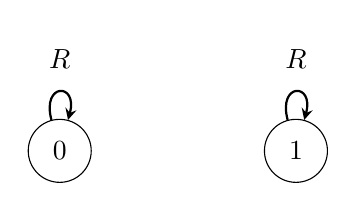
\begin{tikzpicture}[every node/.style={draw, circle, minimum size=8mm}, >=stealth]
\node (a) at (0, 0) {$0$};
\node (b) at (3, 0) {$1$};
\draw[->, thick] (a) to[loop above, looseness=6] node[draw=none, above] {$R$} (a);
\draw[->, thick] (b) to[loop above, looseness=6] node[draw=none, above] {$R$} (b);
\end{tikzpicture}
\par\smallskip{\small A \omterm{def:b2:predicate-logic:structure}{structure} with domain $\{0, 1\}$ and $R$ the equality. Every $y$ has an $x$ with $R(x, y)$,
namely $y$ itself, so $\forall y\, \exists x\, R(x, y)$ is true; no $x$ is related to both $0$ and $1$, so $\exists x\,
\forall y\, R(x, y)$ is false.}
\end{omfigure}

\section{Soundness and completeness}\label{sec:b2:predicate-logic:soundness}

\begin{definition}[Soundness, completeness]\label{def:b2:predicate-logic:soundness}
A proof system is \emph{sound}\index{soundness (proof system)} when every provable \omterm{def:b2:predicate-logic:sequent}{sequent} is a consequence: $\Gamma
\vdash A$ implies $\Gamma \models A$. It is \emph{complete}\index{completeness (proof system)} when every consequence is
provable: $\Gamma \models A$ implies $\Gamma \vdash A$.
\end{definition}

Soundness makes a proof worth having; completeness says that the rules miss nothing. The proof of soundness uses one
fact about \omterm{def:b2:predicate-logic:substitution}{substitution}, which says that substituting a term and changing the assignment are the same operation.

\begin{lemma}[Substitution]\label{lem:b2:predicate-logic:substitution}
For every \omterm{def:b2:predicate-logic:structure}{structure}, assignment $\rho$, \omterm{def:b2:predicate-logic:term}{terms} $s, t$, variable $x$ and formula $A$, with $d = \llbracket t
\rrbracket_\rho$:
\[
\llbracket s[t/x] \rrbracket_\rho = \llbracket s \rrbracket_{\rho[x \mapsto d]}
\qquad\text{and}\qquad
\mathcal{A}, \rho \models A[t/x] \iff \mathcal{A}, \rho[x \mapsto d] \models A.
\]
\end{lemma}

\begin{proof}
For \omterm{def:b2:predicate-logic:term}{terms}, by induction on $s$. If $s$ is $x$, both sides are $d$. If $s$ is another variable $z$, both are $\rho(z)$.
If $s = f(s_1, \dots, s_n)$, then $s[t/x] = f(s_1[t/x], \dots, s_n[t/x])$, and the induction hypothesis on each $s_i$
gives the equality of the arguments, so of the values of $f$. The statement on formulas follows by induction on $A$; its
atomic case is the statement on \omterm{def:b2:predicate-logic:term}{terms}, and its \omterm{def:b2:predicate-logic:formula}{quantifier} case is where capture avoidance is needed
(\cref{exo:b2:predicate-logic:12}).
\end{proof}

The test file \code{test_formulas.py} checks the property on 400 random formulas over a \omterm{def:b2:predicate-logic:structure}{structure} of three elements;
the test fails at once if the renaming of \cref{lst:b2:predicate-logic:subst} is removed.

\begin{theorem}[Soundness of natural deduction]\label{thm:b2:predicate-logic:soundness}
If $\Gamma \vdash A$ has a \omterm{def:b2:predicate-logic:sequent}{proof tree}, then $\Gamma \models A$.
\end{theorem}

\begin{proof}
By induction on the \omterm{def:b2:predicate-logic:sequent}{proof tree}: assuming that the premises of its last rule are consequences, so is its conclusion. Fix
a \omterm{def:b2:predicate-logic:structure}{structure} $\mathcal{A}$ and an assignment $\rho$ satisfying every formula of $\Gamma$; we show $\mathcal{A}, \rho
\models A$ for each rule.
\begin{itemize}
\item \textsc{hyp}: $A \in \Gamma$, and $\rho$ satisfies $\Gamma$.
\item $\wedge$\textsc{i}: by induction $\rho$ satisfies $A$ and $B$, so $A \wedge B$. The eliminations of $\wedge$ and
the introductions of $\vee$ are as direct.
\item $\to$\textsc{e}: $\rho$ satisfies $A \to B$ and $A$, so $B$. The rules $\neg$\textsc{i} and $\neg$\textsc{e} are
the same argument with $\neg A$ read as $A \to \bot$, and $\bot$\textsc{e} holds because no $\rho$ satisfies $\bot$.
\item \textsc{raa}: if $\rho$ did not satisfy $A$, it would satisfy $\Gamma \cup \{\neg A\}$, hence $\bot$ by induction,
which is impossible.
\item $\forall$\textsc{e}: $\rho$ satisfies $\forall x\, A$, so $\rho[x \mapsto \llbracket t \rrbracket_\rho]$ satisfies
$A$, and $\rho$ satisfies $A[t/x]$ by \cref{lem:b2:predicate-logic:substitution}.
\item $\forall$\textsc{i}: let $d \in D$ and $\rho' = \rho[y \mapsto d]$. As $y$ is not \omterm{def:b2:predicate-logic:free}{free} in $\Gamma$, $\rho'$
satisfies $\Gamma$, so by induction it satisfies $A[y/x]$, and by the lemma, with $\llbracket y \rrbracket_{\rho'} = d$,
$\rho'[x \mapsto d]$ satisfies $A$. If $y = x$, this assignment is $\rho[x \mapsto d]$. Otherwise $y$ is not \omterm{def:b2:predicate-logic:free}{free} in
$\forall x\, A$, so not in $A$, and $\rho'[x \mapsto d]$ agrees with $\rho[x \mapsto d]$ on the \omterm{def:b2:predicate-logic:free}{free variables} of $A$. In
both cases $\rho[x \mapsto d]$ satisfies $A$, for every $d$: $\rho$ satisfies $\forall x\, A$.
\end{itemize}
The rules $\to$\textsc{i} and $\vee$\textsc{e} are \cref{exo:b2:predicate-logic:8}, and the rules of $\exists$ follow
the pattern of those of $\forall$.
\end{proof}

The side condition of $\forall$\textsc{i} appears in the proof exactly where it is used: changing $y$ must leave the
hypotheses true. Soundness also gives the method for showing that a \omterm{def:b2:predicate-logic:sequent}{sequent} has no proof. The \omterm{def:b2:predicate-logic:structure}{structure} of the
previous figure satisfies $\forall y\, \exists x\, R(x, y)$ and not $\exists x\, \forall y\, R(x, y)$, so the second is
not a consequence of the first, and by soundness no \omterm{def:b2:predicate-logic:sequent}{proof tree}, however long, derives it.

\begin{theorem}[Completeness]\label{thm:b2:predicate-logic:completeness}
If $\Gamma \models A$, then $\Gamma \vdash A$ has a \omterm{def:b2:predicate-logic:sequent}{proof tree} in \omterm{def:b2:predicate-logic:nd}{natural deduction}.
\end{theorem}

\admitted

The proof builds, from a set of formulas that proves nothing false, a \omterm{def:b2:predicate-logic:structure}{structure} that satisfies all of them, made of the
\omterm{def:b2:predicate-logic:term}{terms} themselves; it is longer than the chapter allows. Together the two theorems say that $\vdash$ and $\models$ are
the same relation. They do not give an algorithm deciding it: one can enumerate all \omterm{def:b2:predicate-logic:sequent}{proof trees}, and if $\Gamma \models
A$ a proof will appear, but if not, the search never ends. No algorithm decides first-order consequence in general; Book 5
develops the methods that prove such impossibility results.

\begin{history}
% ledger: b2:frege-1879
% ledger: b2:gentzen-1935
% ledger: b2:godel-1930
Gottlob Frege published the \emph{Begriffsschrift} in 1879, a formula language for logic modelled on that of
arithmetic, in which quantified variables first appear in their modern role. \omterm{def:b2:predicate-logic:nd}{Natural deduction} and the \omterm{def:b2:predicate-logic:sequent}{sequent} calculus
were introduced by Gerhard Gentzen in a paper of 1935, both to make formal proofs look like the reasoning of
mathematicians; the \omterm{def:b2:predicate-logic:sequent}{sequent} calculus, a variant in which every rule acts on the hypotheses or on the conclusion of a
\omterm{def:b2:predicate-logic:sequent}{sequent}, was the form in which he proved that proofs can be put in a normal form. Kurt Gödel published the completeness
of first-order logic in 1930.
\end{history}

\section{Proof checkers}\label{sec:b2:predicate-logic:checkers}

\begin{definition}[Proof checker]\label{def:b2:predicate-logic:checker}
A \emph{proof checker}\index{proof checker} is a program that, given a \omterm{def:b2:predicate-logic:sequent}{proof tree}, decides whether every node follows
from its children by a rule of the system, side conditions included. If it accepts, the root \omterm{def:b2:predicate-logic:sequent}{sequent} is proved.
\end{definition}

A checker does not search for proofs; it only checks that each step is one of the rules, which is easy. In
\code{checker.py} a proof is a tree of steps, each with its rule, the formula it concludes, the proofs of its premises,
and for the \omterm{def:b2:predicate-logic:formula}{quantifier} rules the variable or term involved. The hypotheses are not stored in the tree:
\code{check} receives them, and passes the extended set to the premises of the rules that add one.

\omcode{code/bachelor-2/24-predicate-logic/listings/checker.py}{60}{92}{The checker's rules for $\vee$, $\to$, $\neg$,
$\bot$ and $\forall$; \code{sub(i, A)} checks premise $i$ with the extra hypothesis $A$}\label{lst:b2:predicate-logic:checker}

\omcode{code/bachelor-2/24-predicate-logic/listings/proofs.py}{20}{28}{Two proofs as data: the proof of
\cref{ex:b2:predicate-logic:forall}, and a $\forall$-introduction on a variable \omterm{def:b2:predicate-logic:free}{free} in the hypothesis}\label{lst:b2:predicate-logic:proofs}

\omoutput{code/bachelor-2/24-predicate-logic/outputs/check_demo.txt}{The four proofs of this chapter are accepted. The
last one is rejected, and the checker names the side condition it breaks.}\label{out:b2:predicate-logic:check-demo}

Each step is checked once, and its checks are comparisons of formulas and \omterm{def:b2:predicate-logic:substitution}{substitutions}, so a checker runs in time
polynomial in the size of the proof. A proof can be enormous and found by any means, by a person, by a search program
or by guessing; it is trusted because a small program, which can itself be read and tested, accepts it.

\begin{dated}{2026}
% ledger: b2:lean
% ledger: b2:rocq
A \emph{proof assistant} is a \omterm{def:b2:predicate-logic:checker}{proof checker} with a language for writing proofs and tools that fill in their routine
steps. Lean is an open-source programming language and proof assistant, with Mathlib, a large library of formalised
mathematics built by its community. The Rocq Prover, formerly the Coq Proof Assistant, is another. Both check proofs in
type theories richer than the logic of this chapter, in which a proof is a program and the formula it proves is its
type.
\end{dated}

\section{Unification and resolution}\label{sec:b2:predicate-logic:resolution}

A program that \emph{searches} for proofs needs a rule that applies blindly. Propositional resolution, from $C \vee L$ and
$C' \vee \neg L$ conclude $C \vee C'$, is such a rule, and a set of clauses is unsatisfiable exactly when it derives the
empty clause. In \omterm{def:b2:predicate-logic:formula}{predicate logic} a clause $\neg \mathit{Out}(x, y) \vee \mathit{Member}(x)$ stands for its universal
closure, and the literal $\mathit{Member}(x)$ should cancel $\neg\mathit{Member}(p5)$ after replacing $x$ by $p5$. The
replacement is found by unification.

\begin{definition}[Unifier, most general unifier, occurs check]\label{def:b2:predicate-logic:unification}
A \omterm{def:b2:predicate-logic:substitution}{substitution} $\sigma$, replacing finitely many variables by \omterm{def:b2:predicate-logic:term}{terms} at the same time, is a
\emph{unifier}\index{unifier} of $s$ and $t$ when $s\sigma = t\sigma$. It is a \emph{most general
unifier}\index{most general unifier} when every unifier $\tau$ is $\sigma$ followed by another \omterm{def:b2:predicate-logic:substitution}{substitution}: $\tau =
\sigma\theta$ for some $\theta$. The \emph{occurs check}\index{occurs check} refuses to bind a variable $x$ to a term
other than $x$ that contains $x$.
\end{definition}

\begin{method}[Robinson's unification]\label{met:b2:predicate-logic:unify}
Keep a list of equations to solve, initially $s = t$, and a \omterm{def:b2:predicate-logic:substitution}{substitution} $\sigma$, initially empty. Repeatedly take an
equation and apply $\sigma$ to both sides. If they are equal, drop it. If one side is a variable $x$: fail if $x$ occurs
in the other side $u$, otherwise add $x \mapsto u$ to $\sigma$. If both are $f(s_1, \dots, s_n)$ and $f(t_1, \dots,
t_n)$ with the same symbol, replace the equation by $s_i = t_i$ for each $i$. Otherwise, with two different symbols,
fail. When the list is empty, return $\sigma$.
\end{method}

\omcode{code/bachelor-2/24-predicate-logic/listings/unify.py}{7}{36}{Unification: \code{walk} applies the bindings found
so far; the \omterm{def:b2:predicate-logic:unification}{occurs check} stops $x = f(x)$}\label{lst:b2:predicate-logic:unify}

\omoutput{code/bachelor-2/24-predicate-logic/outputs/unify_demo.txt}{Four pairs: a \omterm{def:b2:predicate-logic:unification}{unifier} found through a chain of
bindings, a clash of constants, a failed \omterm{def:b2:predicate-logic:unification}{occurs check}, and a second success.}\label{out:b2:predicate-logic:unify}

\begin{theorem}[Robinson]\label{thm:b2:predicate-logic:mgu}
\Cref{met:b2:predicate-logic:unify} terminates. If $s$ and $t$ have a \omterm{def:b2:predicate-logic:unification}{unifier}, it returns a \omterm{def:b2:predicate-logic:unification}{most general unifier};
otherwise it fails.
\end{theorem}

\begin{proof}
Write $\sigma\tau$ for $\sigma$ followed by $\tau$, with $\sigma$ applied until no variable of $\sigma$'s domain is left.
\emph{Invariant}: a \omterm{def:b2:predicate-logic:substitution}{substitution} $\tau$ unifies $s$ and $t$ if and only if $\sigma\tau = \tau$ and $\tau$ solves every
equation of the list. It holds at the start, with $\sigma$ empty.
Dropping an equation with equal sides, or replacing $f(\vec s) = f(\vec t)$ by its arguments, does not change the
solutions. Adding $x \mapsto u$, when $x$ does not occur in $u$, does not either: $\tau$ solves $x = u$ exactly when
$\tau(x) = u\tau$, that is when $x \mapsto u$ followed by $\tau$ is $\tau$.

\emph{Failures}: two different symbols at the roots never become equal under a \omterm{def:b2:predicate-logic:substitution}{substitution}; and if $x$ occurs in $u
\neq x$, then $u\tau$ is strictly larger than $\tau(x)$ for every $\tau$, so $x = u$ has no solution. By the invariant,
$s$ and $t$ then have no \omterm{def:b2:predicate-logic:unification}{unifier}.

\emph{Termination}: a binding removes the variable $x$ from all later equations, since they are walked through $\sigma$,
and the \omterm{def:b2:predicate-logic:unification}{occurs check} ensures it never comes back, so at most as many bindings as variables happen; between two bindings,
each decomposition removes a function symbol from the list, dropping an equation with equal sides removes that
equation, and turning $u = x$ round only changes its order. The triple (number of unbound variables, number of
symbols in the list, variables included, number of equations of the form $u = x$ with $u$ not a variable) decreases at
each step in lexicographic order.

\emph{Result}: when the list is empty, $\sigma$ itself satisfies $\sigma\sigma = \sigma$, since no variable of $\sigma$'s domain
occurs in what $\sigma$ gives, and so by the invariant $\sigma$ unifies $s$ and $t$; every \omterm{def:b2:predicate-logic:unification}{unifier} $\tau$ satisfies
$\sigma\tau = \tau$, so $\sigma$ is most general.
\end{proof}

\begin{definition}[Resolvent, resolution]\label{def:b2:predicate-logic:resolution}
Let $C_1 \vee L_1$ and $C_2 \vee \neg L_2$ be two clauses, their variables renamed so that they share none, with $L_1$
and $L_2$ \omterm{def:b2:predicate-logic:term}{atomic formulas} on the same predicate and $\sigma$ a \omterm{def:b2:predicate-logic:unification}{most general unifier} of $L_1$ and $L_2$. Their
\emph{resolvent}\index{resolvent} is $(C_1 \vee C_2)\sigma$. When two literals $L$ and $L'$ of the same sign in a clause
$C \vee L \vee L'$ have a \omterm{def:b2:predicate-logic:unification}{most general unifier} $\sigma$, the clause $(C \vee L)\sigma$ is a \emph{factor}\index{factor of a clause} of it.
\emph{Resolution}\index{resolution (first-order)} is the proof system with these two rules, resolvents and factors;
a \emph{refutation} of a set of clauses derives the empty clause from it.
\end{definition}

\omcode{code/bachelor-2/24-predicate-logic/listings/unify.py}{60}{68}{\omterm{def:b2:predicate-logic:resolution}{Factors}: two literals of the same sign made
one}

A \omterm{def:b2:predicate-logic:resolution}{resolvent} is a consequence of its two clauses, and a \omterm{def:b2:predicate-logic:resolution}{factor} of its clause, so a refutation proves that the set has no \omterm{def:b2:predicate-logic:consequence}{model}. To prove a goal from
some rules, one refutes the rules together with the negation of the goal. Robinson proved the converse in 1965: a set
of clauses with no \omterm{def:b2:predicate-logic:consequence}{model} has a refutation. His rule resolves several literals at once, which builds factoring in;
binary \omterm{def:b2:predicate-logic:resolution}{resolvents} alone are not enough, and \cref{exo:b2:predicate-logic:3} gives two clauses with no \omterm{def:b2:predicate-logic:consequence}{model} from
which they never reach the empty clause. A whole proof is found by trying all pairs, as \code{refute.py} does for ``p5
may borrow'':

\omoutput{code/bachelor-2/24-predicate-logic/outputs/refute.txt}{\omterm{def:b2:predicate-logic:resolution}{Resolution} proves that \code{p5} may borrow. Each new
clause names its two parents and the \omterm{def:b2:predicate-logic:unification}{unifier}; clause (5) chains the two rules into one before any fact is
used.}\label{out:b2:predicate-logic:refute}

% ledger: b2:robinson-1965
Robinson published unification and resolution together in 1965, for a logic oriented towards machines rather than
towards people. \omterm{def:b2:predicate-logic:resolution}{Resolution} on clauses with at most one positive literal, Horn clauses, is the engine of logic
programming, and unification reappears in Book 5, where the types of a program are inferred by solving equations
between type \omterm{def:b2:predicate-logic:term}{terms}.

\section{2-SAT and the implication graph}\label{sec:b2:predicate-logic:2sat}

Satisfiability has a case solved in linear time. For three literals per clause no algorithm much faster than the
search of the Year 1 volume is known; with two, each clause is a pair of implications.

\begin{definition}[Implication graph]\label{def:b2:predicate-logic:implication-graph}
The \emph{implication graph}\index{implication graph} of a 2-CNF formula over $x_1, \dots, x_n$ is the directed graph
whose $2n$ vertices are the literals $x_k$ and $\neg x_k$, with two edges $\neg a \to b$ and $\neg b \to a$ for each
clause $a \vee b$ (where $\neg\neg x$ is $x$).
\end{definition}

An edge $\ell \to m$ says that every \omterm{def:b2:predicate-logic:consequence}{model} making $\ell$ true makes $m$ true, so a path does too. The formula $(x_1 \vee
x_2) \wedge (\neg x_1 \vee x_2) \wedge (x_1 \vee \neg x_2) \wedge (\neg x_1 \vee \neg x_2)$ forbids each of the four
assignments, and its graph has a single strongly connected component:

\begin{omfigure}
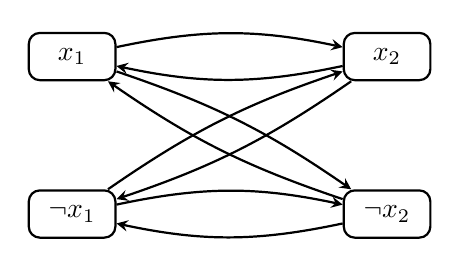
\begin{tikzpicture}[every node/.style={draw, rounded corners, minimum width=11mm, minimum height=6mm}, >=stealth,
thick]
\node (a) at (0, 2) {$x_1$};
\node (b) at (4, 2) {$x_2$};
\node (na) at (0, 0) {$\neg x_1$};
\node (nb) at (4, 0) {$\neg x_2$};
\draw[->] (a) to[bend left=12] (b);
\draw[->] (b) to[bend left=12] (a);
\draw[->] (na) to[bend left=12] (nb);
\draw[->] (nb) to[bend left=12] (na);
\draw[->] (na) to[bend left=8] (b);
\draw[->] (b) to[bend left=8] (na);
\draw[->] (nb) to[bend left=8] (a);
\draw[->] (a) to[bend left=8] (nb);
\end{tikzpicture}
\par\smallskip{\small The \omterm{def:b2:predicate-logic:implication-graph}{implication graph} of the four clauses on $x_1, x_2$: each clause $a \vee b$ gives the edges
$\neg a \to b$ and $\neg b \to a$. All four literals are in one strongly connected component, so $x_1$ implies $\neg
x_1$ and $\neg x_1$ implies $x_1$.}
\end{omfigure}

\begin{theorem}[2-SAT in linear time]\label{thm:b2:predicate-logic:2sat}
A 2-CNF formula is unsatisfiable if and only if, for some variable $x$, the literals $x$ and $\neg x$ lie in the same
strongly connected component of its \omterm{def:b2:predicate-logic:implication-graph}{implication graph}. Satisfiability, and a \omterm{def:b2:predicate-logic:consequence}{model} when there is one, are found in time
linear in the number of variables and clauses.
\end{theorem}

\begin{proof}
If $x$ and $\neg x$ share a component, there are paths $x \leadsto \neg x$ and $\neg x \leadsto x$. A \omterm{def:b2:predicate-logic:consequence}{model} making $x$
true makes $\neg x$ true along the first, and one making $x$ false makes $x$ true along the second: there is no \omterm{def:b2:predicate-logic:consequence}{model}.

Conversely, suppose no variable shares a component with its negation. Number the components in a topological order of
the graph of components, so that every edge goes from a component to the same or a later one, and write $c(\ell)$ for
the number of the component of $\ell$. Make $\ell$ true when $c(\ell) > c(\neg \ell)$; exactly one of $x$, $\neg x$ is
true since their numbers differ. Suppose a clause $a \vee b$ had both literals false: $c(a) < c(\neg a)$ and $c(b) <
c(\neg b)$. The edges $\neg a \to b$ and $\neg b \to a$ give $c(\neg a) \leq c(b)$ and $c(\neg b) \leq c(a)$, so $c(a) <
c(\neg a) \leq c(b) < c(\neg b) \leq c(a)$, a contradiction. The assignment is a \omterm{def:b2:predicate-logic:consequence}{model}.

The graph has $2n$ vertices and twice as many edges as clauses; Kosaraju's algorithm finds its components in linear
time, and numbers them in a topological order as it goes.
\end{proof}

\omcode{code/bachelor-2/24-predicate-logic/listings/twosat.py}{5}{16}{The \omterm{def:b2:predicate-logic:implication-graph}{implication graph}: two edges per clause, and
the reversed edges for the second search of Kosaraju's algorithm}\label{lst:b2:predicate-logic:twosat}

\omcode{code/bachelor-2/24-predicate-logic/listings/twosat.py}{44}{49}{The test of \cref{thm:b2:predicate-logic:2sat},
and the \omterm{def:b2:predicate-logic:consequence}{model} read from the order of the components}\label{lst:b2:predicate-logic:twosat-model}

The talks of a two-room meeting are a 2-SAT instance: $x_k$ says that talk $k$ is in the big room, two talks with a
speaker in common must be in different rooms ($x_j \vee x_k$ and $\neg x_j \vee \neg x_k$), and a talk that needs the
big room's screen gives the clause $x_k \vee x_k$.

\omoutput{code/bachelor-2/24-predicate-logic/outputs/twosat_demo.txt}{A plan for the five talks, then none once a sixth
talk shares speakers with talk 4 and cannot be in the big room with talk 1; all 64 assignments confirm both. Talk 6 is
in no clause of the first formula, so its one plan counts twice: $2 = 1 \times 2$.}\label{out:b2:predicate-logic:twosat}

% ledger: b2:aspvall-1979
The algorithm is due to Bengt Aspvall, Michael Plass and Robert Tarjan, in 1979. It is the reason why 2-SAT, unlike
3-SAT, appears inside other algorithms as a routine step.

\section{Exercises}\label{sec:b2:predicate-logic:exercises}

\begin{exercise}[$\star$]\label{exo:b2:predicate-logic:1}
Give the \omterm{def:b2:predicate-logic:free}{free variables} of $\forall x\, R(x, y)$; $(\forall x\, P(x)) \to P(x)$; $\exists x\, \forall y\, R(x, y)
\wedge R(y, z)$; $\forall x\, ((\exists x\, P(x)) \to Q(x, f(y)))$; $\exists y\, (y = f(x) \wedge \forall x\, \neg R(x,
y))$. Then run \code{exo_free.py} and compare.
\end{exercise}

\begin{exercise}[$\star$]\label{exo:b2:predicate-logic:2}
The function \code{replace} of \code{exo_capture.py} is meant to compute $A[t/x]$. Which of its three results is wrong,
and why? Correct the function.
\end{exercise}

\begin{exercise}[$\star$]\label{exo:b2:predicate-logic:3}
Predict the result of unifying $P(f(x), y)$ with $P(y, f(a))$; $P(x, f(x))$ with $P(f(y), y)$; $P(x, y, z)$ with $P(y,
z, a)$; $P(g(x), x)$ with $P(f(y), a)$. Check with \code{exo_unify.py}. Then show that the two clauses $P(x) \vee
P(y)$ and $\neg P(x) \vee \neg P(y)$ have no \omterm{def:b2:predicate-logic:consequence}{model}, that binary \omterm{def:b2:predicate-logic:resolution}{resolvents} alone, however often repeated,
only ever give clauses of two literals, and find a refutation that uses \omterm{def:b2:predicate-logic:resolution}{factors}. Check with \code{factor_demo.py}.
\end{exercise}

\begin{exercise}[$\star$]\label{exo:b2:predicate-logic:4}
Draw the \omterm{def:b2:predicate-logic:implication-graph}{implication graph} of $(x_1 \vee x_2) \wedge (\neg x_1 \vee x_3) \wedge (\neg x_2 \vee \neg x_3) \wedge (\neg x_3
\vee x_1)$ and find its strongly connected components. Is the formula satisfiable? What changes when the clause $\neg
x_1 \vee \neg x_3$ is added, and then also $x_1 \vee x_3$? Check with \code{exo_twosat.py}.
\end{exercise}

\begin{exercise}[$\star\star$]\label{exo:b2:predicate-logic:5}
For the three \omterm{def:b2:predicate-logic:free}{sentences} $\forall x\, \exists y\, R(x, y)$, $\neg \exists x\, R(x, x)$ and $\exists y\, \forall x\, \neg
R(x, y)$, say which hold in: $\mathbb{Z}/3$ with $R(x, y)$ when $y = x + 1$; $\{0, 1, 2\}$ with $R$ the order $<$;
$\{0, 1\}$ with $R$ the relation $\neq$. Check with \code{exo_three.py}.
\end{exercise}

\begin{exercise}[$\star\star$]\label{exo:b2:predicate-logic:6}
The checker rejects the proof of \code{exo_forall_bug.py}. Is its conclusion a consequence of its hypotheses? Give a
\omterm{def:b2:predicate-logic:structure}{structure} that answers, then the strongest correct conclusion its steps support.
\end{exercise}

\begin{exercise}[$\star\star$]\label{exo:b2:predicate-logic:7}
Write a \omterm{def:b2:predicate-logic:sequent}{proof tree} of $\neg(P \vee Q) \vdash \neg P \wedge \neg Q$, then write it as data for the checker.
\end{exercise}

\begin{exercise}[$\star\star$]\label{exo:b2:predicate-logic:8}
Complete the proof of \cref{thm:b2:predicate-logic:soundness} with the cases of $\to$\textsc{i} and $\vee$\textsc{e}.
\end{exercise}

\begin{exercise}[$\star\star$]\label{exo:b2:predicate-logic:9}
Extend the checker with the rules $\exists$\textsc{i} and $\exists$\textsc{e}, through its argument \code{extra}, which
maps a rule's name to a function receiving the step, the hypotheses, \code{sub} and \code{need}.
\end{exercise}

\begin{exercise}[$\star\star\star$]\label{exo:b2:predicate-logic:10}
Prove $\exists x\, \forall y\, R(x, y) \vdash \forall y\, \exists x\, R(x, y)$ and check the proof with
\cref{exo:b2:predicate-logic:9}. Try the same plan for the converse: which side condition stops it, and why must
something stop it?
\end{exercise}

\begin{exercise}[$\star\star\star$]\label{exo:b2:predicate-logic:11}
Prove $\vdash P \vee \neg P$ in \omterm{def:b2:predicate-logic:nd}{natural deduction}, and check the proof. Explain why every proof of it uses
\textsc{raa}: find a reading of the rules other than \textsc{raa} under which each rule preserves a property that $P \vee
\neg P$ lacks, or argue from the shape of a proof that ends with $\vee$\textsc{i}.
\end{exercise}

\begin{exercise}[$\star\star\star$]\label{exo:b2:predicate-logic:12}
Prove the formula part of \cref{lem:b2:predicate-logic:substitution} by induction on $A$, with the \omterm{def:b2:predicate-logic:substitution}{substitution} of
\cref{lst:b2:predicate-logic:subst}. Where is the renaming used?
\end{exercise}

\section{Problem: Checking the library's rules}\label{sec:b2:predicate-logic:problem}

\begin{problem}[{Weekend problem --- Checking the library's rules}]\label{pb:b2:predicate-logic:1}
The library keeps three rules: $H_1$, whoever has a book out is a member; $H_2$, every member may borrow; $H_3$, a book
that is out has been borrowed by that person. It would like to know which other rules follow from them: $C_1$, whoever
has a book out may borrow; $C_2$, whoever has a book out is a member and has borrowed it; $C_3$, whoever may not borrow
is not a member; $C_4$, every member has a book out.

\omcode{code/bachelor-2/24-predicate-logic/listings/library.py}{10}{32}{The three rules and the proof of $C_1$, as data
for the checker}\label{lst:b2:predicate-logic:library}

\omoutput{code/bachelor-2/24-predicate-logic/outputs/library.txt}{Three consequences proved and checked; the fourth
refuted by a \omterm{def:b2:predicate-logic:structure}{structure} found among the 4096 on two elements.}\label{out:b2:predicate-logic:library}

\needspace{4\baselineskip}\medskip\noindent\textbf{Part I --- The rules as sentences.}\par\nopagebreak
\begin{enumerate}
\item Write $H_1$, $H_2$, $H_3$ and $C_1$ to $C_4$ as \omterm{def:b2:predicate-logic:free}{sentences} over $\mathit{Out}$, $\mathit{Member}$,
$\mathit{MayBorrow}$ and $\mathit{Borrowed}$.
\item $H_1$ is written $\forall x\, \forall y\, (\mathit{Out}(x, y) \to \mathit{Member}(x))$ in the program, and
$\forall x\, ((\exists y\, \mathit{Out}(x, y)) \to \mathit{Member}(x))$ in \cref{lst:b2:predicate-logic:evaluate}. Prove
that the two are equivalent.
\item What are the \omterm{def:b2:predicate-logic:free}{free variables} of $\mathit{Out}(x, y) \to \mathit{Member}(x)$? Why must the rules be \omterm{def:b2:predicate-logic:free}{sentences}?
\item Write ``a book is out to one person at most'' as a \omterm{def:b2:predicate-logic:free}{sentence}, and explain each \omterm{def:b2:predicate-logic:formula}{quantifier}.
\item The \omterm{def:b2:predicate-logic:free}{sentence} $\forall x\, \exists y\, \mathit{Out}(x, y) \to \mathit{Member}(x)$ is not $H_1$. Put its brackets and
say what it means.
\item How many nested \omterm{def:b2:predicate-logic:formula}{quantifiers} do $C_2$ and the rule of question 4 have, and what does
\cref{prop:b2:predicate-logic:evaluation-cost} predict for their cost on the town?
\end{enumerate}

\needspace{4\baselineskip}\medskip\noindent\textbf{Part II --- The rules on the town's data.}\par\nopagebreak
\begin{enumerate}[resume, beginpenalty=10000]
\item Which of the five rules of \cref{lst:b2:predicate-logic:evaluate} hold in the town?
\item The rule ``out to one person at most'' has 8 counterexamples. Why 8, for 4 books?
\item What does a counterexample to that rule say about the loans table, and what should the library do about it?
\item The rule ``every member has a friend'' fails 41 times. Is this an error in the data?
\item Why does the town satisfy $H_1$ and $H_3$ although nobody proved them about the town?
\item Rewrite the rule of question 4 as a search for its counterexamples by one pass over the loans, and give its cost.
\end{enumerate}

\needspace{4\baselineskip}\medskip\noindent\textbf{Part III --- Proofs in natural deduction.}\par\nopagebreak
\begin{enumerate}[resume, beginpenalty=10000]
\item Draw the \omterm{def:b2:predicate-logic:sequent}{proof tree} of $C_1$ from \cref{lst:b2:predicate-logic:library}.
\item Why are the two uses of $\forall$\textsc{i} in the proof of $C_1$ allowed?
\item Write a proof of $C_2$ that uses the proof of $\mathit{Out}(x, y) \vdash \mathit{Member}(x)$ as a part.
\item Write a proof of $C_3$. Which rule for $\neg$ does it use, and which hypothesis does it discharge?
\item Count the steps of your proof of $C_1$ and compare with the output.
\item The proof of $C_1$ proves the \omterm{def:b2:predicate-logic:sequent}{sequent} for $x$ and $y$ and then generalises. Why can it not instead prove
$\mathit{MayBorrow}(p5)$ and generalise from $p5$?
\end{enumerate}

\needspace{4\baselineskip}\medskip\noindent\textbf{Part IV --- Checked mechanically, and a countermodel.}\par\nopagebreak
\begin{enumerate}[resume, beginpenalty=10000]
\item What does the checker's acceptance of $C_1$ to $C_3$ prove, by \cref{thm:b2:predicate-logic:soundness}?
\item Describe the \omterm{def:b2:predicate-logic:structure}{structure} found for $C_4$ in words: a library, a member, no loan.
\item Why does this \omterm{def:b2:predicate-logic:structure}{structure} prove that no proof of $C_4$ from $H_1$ to $H_3$ exists?
\item Is there a countermodel with a domain of one element? Why did the program search two?
\item The program tries \omterm{def:b2:predicate-logic:structure}{structures} in a fixed order. How many \omterm{def:b2:predicate-logic:structure}{structures} on two elements are there for these four
predicates, and how long would the search take on three elements?
\item Prove $C_1$ by resolution, writing $H_1$, $H_2$ and the negation of $C_1$ as clauses, and state the result: 3
rules proved in 34 checked steps, and a two-element countermodel for the one that does not follow.
\end{enumerate}
\end{problem}
